\documentclass{beamer}
\usetheme{metropolis}           % Use metropolis theme
\title{ Adversarial Learning}
\date{\today}
\author{Kacper}
\institute{}
\begin{document}
  \maketitle
  
  
  
\begin{frame}{Learning density}
The aim is to learn distribution $p$.
We want to  learn a generative model $G$, such that for a random variable $Z$, $G(Z) \sim p$.
Or, $p = p_G$, where $p_G$ is distribution of $G(Z)$.
\end{frame}
  
\section{Generative Adversarial Networks}
  
\begin{frame}{artificial  labels}
  \begin{itemize}
   \item Random variable  $X$, distributed according to distribution $p$. 
   \item Some noise random variable $Z$.
   \item A generative model $G$, which transforms $Z$ to $X' = G(Z)$, in other words  $X' \sim p_{G}$.
\end{itemize}

Consider an artificial  label   $Y \in \{ -1,1 \}$, distributed according to Bernoulli distribution. 
Consider a random vector $W$, such that $W_1 = Y$.  

if $Y=1$  then  $W_2 =X \sim p$.

if $Y=-1$  then $W_2 =X' \sim p_G$.

I probably could have written $W  = (1,X) | (-1,X')$.

\end{frame}
  
  
   
\begin{frame}{Classifier}

Let $D$ be discriminative function which is suppose to figure out if $W_2$ comes from $p$ or $p_G$ (if $W_2 = X'$ or $W_2=X$). 

For a random variable  $V$,  $D(W_2)$ a probability that $W_1 =1$ (label is one).  

\end{frame}
  
  
  
  
\begin{frame}{Learning density}

Consider an expression  
$$
E \left( \log(D(W_2)) | Y=1 \right)  + E \left( \log(1 - D(W_2))| Y=-1  \right).
$$
It can be written using $X$,$G(Z)$, as a function of $D,G$
$$
V(D,G) = E \log(D(X)) + E \log(1 - D(G(Z)))
$$
For each generator  $G$ there exists an optimal  discriminator $D$ that maximizes the above function (we will show). 
$$C(G) = \sup_{D} V(D,G)$$

We are going to show that $G$ that minimizes $C(G)$ is the best generator, i.e. $p_G = p$.
\end{frame}
  
\begin{frame}{Optimal discriminator}
For each generator  $G$ there exists an optimal  discriminator $D$ that maximizes the above function (as we will show).
\begin{align}
V(D,G) =& E \left[ \log D(X) +  \log(1 - D(G(Z)))  \right] \\ 
       =& E\left[  \log D(X) +  \log(1 - D(X')) \right] \\
       =& \int p(x)  \log D(x) +  p_G(x) \log(1 - D(x))
\end{align}
which, for a fixed $G$, $V(D,G)$ reaches  maximum  at $D = \frac{p}{p+p_g}$


\end{frame}
\begin{frame}{Experiments}
All the experimatal reasults will be discussed at the end.
 
\end{frame}


  
\begin{frame}{Optimal generator }
For a fixed, optimal $D = \frac{p}{p+p_g} $, $V$ is a divergence 
\begin{align}
V(D,G) =& E \left(  \log D(X) + \log(1 - D(X')) \right) \\ 
&E \left(   \log \frac{p(X)}{p(X)+p_g(X)} + \log \frac{p_g(X')}{p(X')+p_g(X')} \right) =\\
&D_{KL}(p || \frac{p+p_g}{2} ) + D_{KL}(p_g ||  \frac{p+p_g}{2})
\end{align}

\end{frame}  


\section{Training generative neural networks via Maximum Mean Discrepancy optimization}

\begin{frame}{Relating to distance between measures}
The discriminator presented in the previous paper was $C(G) = \sup_{D} V(D,G)$. This paper suggests to put 
\[
 C(G) = MMD(G(Z),X) 
\]
and the rest remains the same, we solve 
\begin{align}
\arg \min C(G)
\end{align}
\end{frame}

\begin{frame}{Deatils}
Suppose  $\theta$ is parameter  of the network $G$. The gradient of MMD  w.r.t. to $\theta$ on the  smallest minibatch batch 
$y_1 = G(z_1), y_2 = G(z_2),x_1,x_2$, is

\begin{align*}
\nabla MMD \sim & \frac{ \partial k(y_1,y_2) } {\partial (y_1,y_2) } (\frac{\partial y_1}{\partial \theta } ,\frac{ \partial y_2} {\partial \theta }) + \\
   &-\frac{ \partial k(x_1,y_1) }{2\partial y_1} \frac{\partial y_1}{\partial \theta } -  \frac{ \partial k(x_2,y_1) }{2\partial y_1} \frac{\partial y_1}{\partial \theta }+ \\
   & -\frac{ \partial k(x_1,y_2) }{2\partial y_1} \frac{\partial y_1}{\partial \theta } - \frac{ \partial k(x_2,y_2) }{2\partial y_1} \frac{\partial y_1}{\partial \theta }
 \end{align*}


\end{frame}
 



\begin{frame}{Training algortihm}
\begin{figure}
 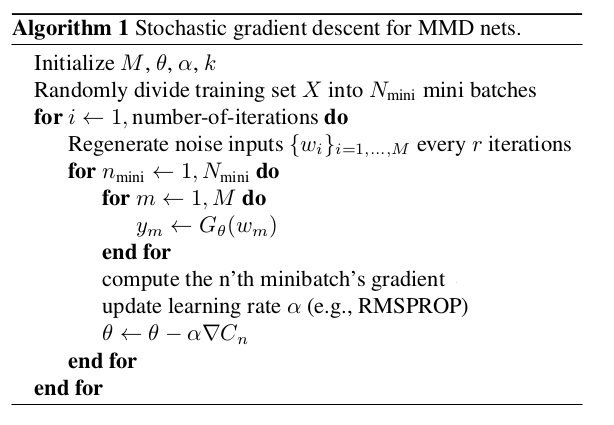
\includegraphics[width=\textwidth]{./img/alg1.png}
\end{figure}
\end{frame}  

\begin{frame}{Comments}
Arthur noticed that varaince of MMD should be taken into account in the objective i.e. 
\[
 \frac{ \overline{MMD}}{ \sqrt{ var(\overline{MMD})}}.
\]

Are random variables suitable model for images? 
'It is well known that, for any distribution $p$ and any continuous distribution $p_z$ on sufficiently regular spaces (...), there is a function $G$, such that $G(Z)$'
\end{frame}

% \begin{frame}{Why images might be dificult to generate from a noise}
% \begin{figure}
% 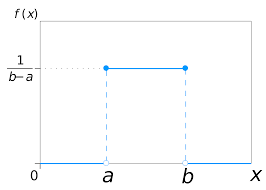
\includegraphics[width=0.3\textwidth]{./img/uni.png}\\
% \end{figure}
% \begin{figure}
% 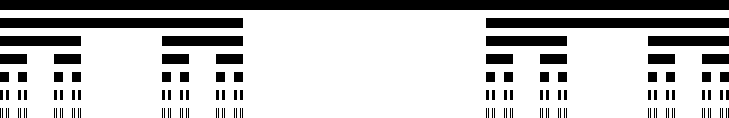
\includegraphics[width=\textwidth]{./img/Cantor.png}  
% \end{figure}
% 

 

% \label{By 127 "rect" - From en.wikipedia.org }
% \end{frame}


\section{Deep Mean Maps, digression}
\begin{frame}{Not excatly what I've expected}
 Use random features  as a layer in a network, $L^i$ is a layer for $i$-th picture  
 $$
 L^i \in R^{H,W}
 $$
 $H,W$ is number of (super) pixels. For frequencies $\omega_1, \cdots,\omega_d,\cdots,\omega_D$, use feature in network
 $$
 \mu^i_d = \sum_{w=1,h=1}^{H,W} \cos(\omega_d L^i_{h,w}+b) ) 
 $$
\end{frame}



\section{Deep Generative Image Models using a Laplacian Pyramid of Adversarial Networks}

\begin{frame}{The conditional generative adversarial net}
$D$ receives  additional  information $L$ as input. This might contain, say, information about the class of the training example
$X$.
\[
\arg \min_{G} \sup_{D} E \log(D(X,L)) + E \log(1 - D(G(Z),L))
\] 
M. Mirza and S. Osindero. Conditional generative adversarial nets.
\end{frame}


\begin{frame}{Laplacian Pyramid}
$d$ is downsampling operation which blurs and decimates a $j\times j$ image $I$ to $d(I)$, which is $j/2 \times j/2$.
$u$ is upsampling opertation that which smooths and expands.
$I_k = d^k(I)$
$h_k$ are residuals i.e $h_k = I_k - u(d(I_k))$.
They aim to lear residuals.
\end{frame}

\begin{frame}{Sampling}
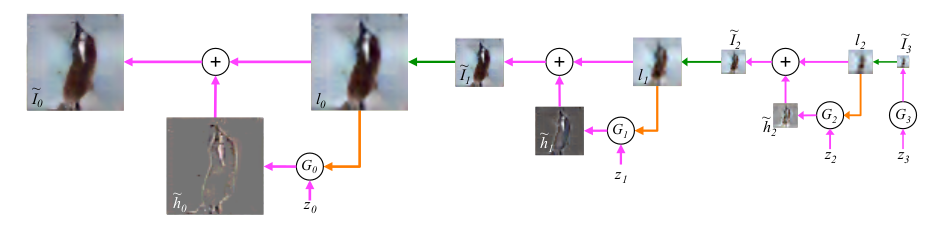
\includegraphics[width=\textwidth]{./img/sampling.png}
\end{frame}

\begin{frame}{Learning}
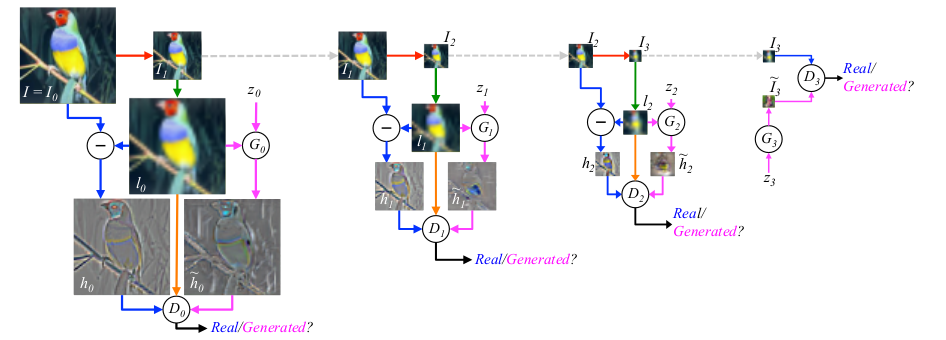
\includegraphics[width=\textwidth]{./img/learning.png}
\end{frame}

\section{Resluts}

\begin{frame}{GAN}
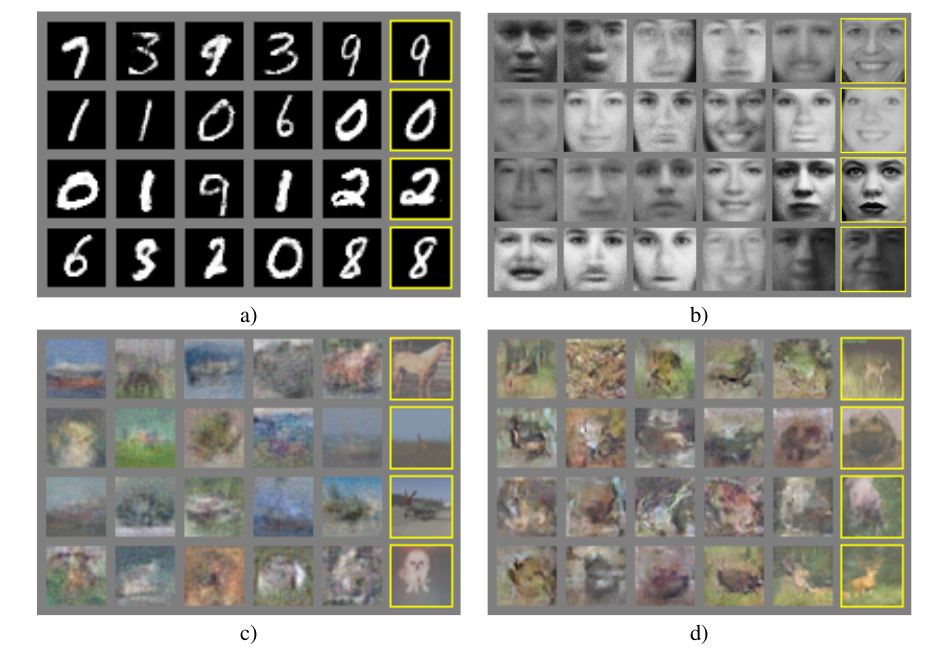
\includegraphics[width=\textwidth]{./img/ganRes.png}

a) MNIST b) TFD c) CIFAR-10 (fully connected model) d) CIFAR-10 (convolutional discriminator
and “deconvolutional” generator)
\end{frame}

\begin{frame}{MMD}
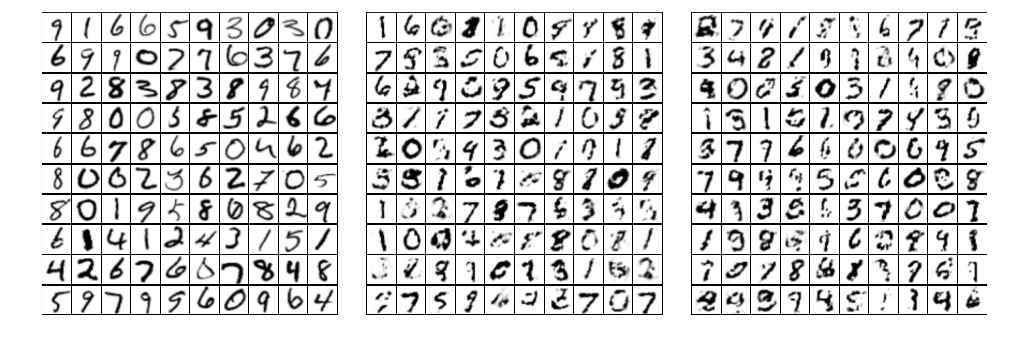
\includegraphics[width=\textwidth]{./img/mmd.png}

MNIST
\end{frame}


\begin{frame}{LAPGAN}
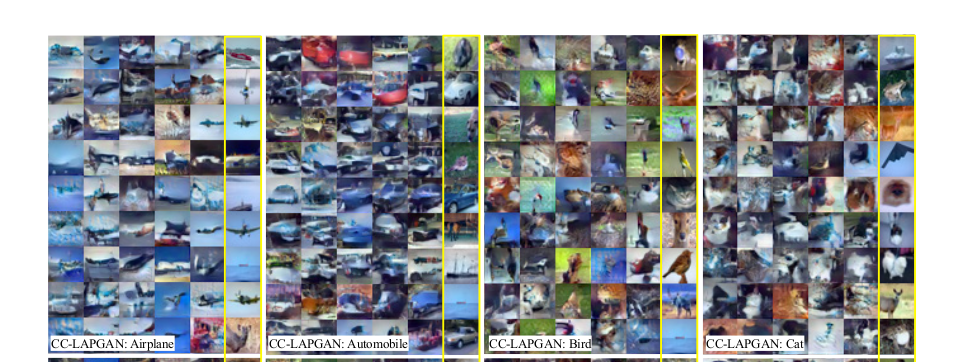
\includegraphics[width=\textwidth]{./img/CIFAR-Lap.png}

CIFAR 10
\end{frame}



\begin{frame}{LAPGAN}
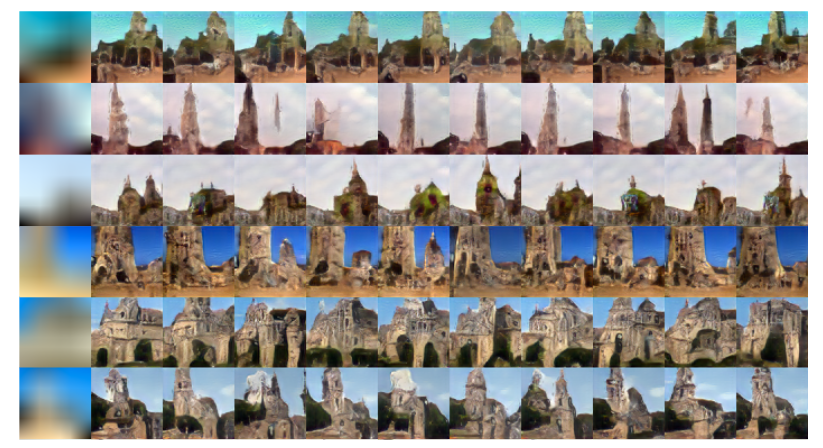
\includegraphics[width=\textwidth]{./img/LSUN.png}

LSUN
\end{frame}

\end{document}